\documentclass[11pt]{article}
\usepackage{fullpage}
\usepackage{amsmath, amssymb, bigints, graphicx}

\title{Classical Lamination Theory \\
      { \normalsize ~ \\ A note in support of \textit{Fiber Orientation Tools} \\
       \texttt{http://github.com/charlestucker3/Fiber-Orientation-Tools}}}

\author{Charles L.~Tucker III \\
       Department of Mechanical Science and Engineering \\
        University of Illinois at Urbana-Champaign \\
        1206 W.~Green St. \\
        Urbana, IL 61801 \\
        }
% Definitions and declarations for "Fundamentals of Fiber Orientation" by C. L. Tucker

\DeclareMathOperator{\tr}{tr}   % Math operator for the trace of tensor (must be in the preamble)

% Math shortcuts j
\newcommand{\ud}{\mathop{}\!\mathrm{d}}  % Roman d as the differential operator,  no space after
\newcommand{\uD}{\mathop{}\!\mathrm{D}}  % Roman D as the differential operator for D/Dt
\newcommand{\A}{\ensuremath{\mathbf{A}}}          % Second-order orientation tensor, direct notation
\newcommand{\Afour}{\ensuremath{\mathbb{A}}}  % Fourth-order orientation tensor
\newcommand{\B}{\ensuremath{\mathbf{B}}}           % Piola tensor, direct notation
\newcommand{\Bfour}{\ensuremath{\mathbb{B}}}   % Fourth-order strain concentration tensor 
\newcommand{\C}{\ensuremath{\mathbf{C}}}          % Fiber-fiber interaction tensor in ARD models
\newcommand{\Cfour}{\ensuremath{\mathbb{C}}}  % Fourth-order stiffness tensor
\newcommand{\D}{\ensuremath{\mathbf{D}}}          % Rate-of-deformation tensor, direct notation
\newcommand{\Efour}{\ensuremath{\mathbb{E}}}   % Fourth-order Eshelby tensor
\newcommand{\F}{\ensuremath{\mathbf{F}}}            % Deformation gradient tensor, direct notation
\newcommand{\Ffour}{\ensuremath{\mathbb{F}}}    % Arbitrary fourth-order tensor (Appendix A) 
\newcommand{\Gfour}{\ensuremath{\mathbb{G}}}   % Arbitrary fourth-order tensor (Appendix A)  
\newcommand{\Hfour}{\ensuremath{\mathbb{H}}}   % Fourth-order strain concentration, Eshelby dilute model 
\newcommand{\Ifour}{\ensuremath{\mathbb{I}}}   % Fourth-order identity tensor
\newcommand{\jv}{\ensuremath{\mathbf{j}}}           % j vector (bold) for particle flux
\newcommand{\Lfour}{\ensuremath{\mathbb{L}}}   % Fourth-order L tensor (RSC model)
\newcommand{\Lub}{\ensuremath{L_\mathrm{ub}}} % Unbreakable fiber length L_ub
\newcommand{\Mfour}{\ensuremath{\mathbb{M}}}  % Fourth-order M tensor (RSC model)
\newcommand{\St}{\ensuremath{\mathbf{S}}}          % Arbitrary second-order tensor (Appendix A) 
\newcommand{\T}{\ensuremath{\mathbf{T}}}          % Arbitrary second-order tensor (Appendix A) 
\newcommand{\Tfour}{\ensuremath{\mathbb{T}}}  % Arbitrary fourth-order tensor, groupFlow chapter
\newcommand{\W}{\ensuremath{\mathbf{W}}}        % Vorticity, direct notation
\newcommand{\ev}{\ensuremath{\mathbf{e}}}         % e vector, bold
\newcommand{\fv}{\ensuremath{\mathbf{f}}}         % f vector, bold
\newcommand{\pv}{\ensuremath{\mathbf{p}}}         % p vector, bold
\newcommand{\mv}{\ensuremath{\mathbf{m}}}         % m vector, bold
\newcommand{\nv}{\ensuremath{\mathbf{n}}}         % n vector, bold
\newcommand{\qv}{\ensuremath{\mathbf{q}}}         % q vector, bold
\newcommand{\Rfour}{\ensuremath{\mathbb{R}}}  % 6x6 matrix used in fourth-order contracted notation 
\newcommand{\Sfour}{\ensuremath{\mathbb{S}}}   % Fourth-order compliance tensor 
\newcommand{\tv}{\ensuremath{\mathbf{t}}}          % t vector, bold
\newcommand{\uv}{\ensuremath{\mathbf{u}}}          % u vector, bold
\newcommand{\xv}{\ensuremath{\mathbf{x}}}          % x vector, bold
\newcommand{\vf}{\ensuremath{\phi_{f}}}                 % v_f (fiber volume fraction) with some kerning of the f
\newcommand{\vm}{\ensuremath{\phi_m}}                 % v_m (matrix volume fraction) 
\newcommand{\vv}{\ensuremath{\mathbf{v}}}          % v vector, bold
\newcommand{\dv}{\ensuremath{\skew{4} \hat{\boldsymbol{\delta}}}}  % delta-hat unit vector, bold
\newcommand{\jj}{\ensuremath{j}}                          % use in subscripts for better kerning of j
\newcommand{\ff}{\ensuremath{f}}                          % use in subscripts for better kerning of f
\newcommand{\epsilondotP}{\ensuremath \dot{\varepsilon}_{\! \scriptscriptstyle P}}  % epsilon-dot sub-P
\newcommand{\epsilondotB}{\ensuremath \dot{\varepsilon}_{\! \scriptscriptstyle B}}  % epsilon-dot sub-B
\newcommand{\epsilondotU}{\ensuremath \dot{\varepsilon}_{\! \scriptscriptstyle U}}  % epsilon-dot sub-U
\newcommand{\balpha}{\ensuremath{\boldsymbol{\alpha}}}                  % bold alpha, thermal expansion tensor
\newcommand{\bbeta}{\ensuremath{\boldsymbol{\beta}}}                      % bold beta, thermal stress tensor
\newcommand{\bepsilon}{\ensuremath{\boldsymbol{\varepsilon}}}       % bold epsilon, small strain tensor
\newcommand{\bsigma}{\ensuremath{\boldsymbol{\sigma}}}                  % sigma (total stress tensor), bold
\newcommand{\bSigma}{\ensuremath{\boldsymbol{\Sigma}}}                 % cap Sigma, bold
\newcommand{\btau}{\ensuremath{\boldsymbol{\tau}}}                           % tau (extra stress tensor), bold
\newcommand{\etaI}{\ensuremath \eta_{\scriptscriptstyle I}}                                         % eta sub-I
\newcommand{\elli}{\ensuremath \ell_{i}}                                                                       % ell sub-i
\newcommand{\omegav}{\ensuremath{\boldsymbol{\omega}}}              % bold omega, for angular velocity
\newcommand{\matlab}{\textsc{Matlab}}                   % "Matlab" in small caps
\newcommand{\nablasurf}{\ensuremath{\nabla_{s}}}    % surface gradient operator, w/ _s kerned


  % Macro definitions

\begin{document}
\maketitle

The function \texttt{Clayer2laminate} in \emph{Fiber Orientation Tools} uses classical lamination theory to find the stiffness properties of a composite where the fiber orientation, fiber volume fraction, and/or the fiber length distribution vary across the thickness.  Such structures are typical for injection molded composites.  

This note explains the nomenclature used by \texttt{Clayer2laminate} and summarizes the underlying theory.  We develop the laminate properties in a notation  that is common in the structural mechanics of laminated composite materials\footnote{E.g., R. M. Jones, \emph{Mechanics of Composite Materials}. Taylor \& Francis, Philadelphia, 2nd edition, 1999.}.  Equation numbers with a period, e.g., Eqn.~(8.2), and section numbers refer to items from \emph{Fundamentals of Fiber Orientation}, C. L. Tucker, Hanser, Munich, 2022.  

\subsection*{Coordinate System}

In the language of laminated composites, a \emph{laminate} is a plate-like structure consisting of multiple discrete layers, or \emph{lamina}, bonded together.  Choose $(x,y,z)$ coordinates so that $z = 0$ is the midplane of the laminate, and let the total thickness of the laminate be $H$.  

\subsection*{Strains and Curvatures}

Let the components of the displacement vector be $(u, v, w)$.  The components of the strain tensor follow from the usual definitions, e.g., Eqns.~(8.2) and (8.3):
\begin{equation}
   \varepsilon_{xx} = \frac{\partial u}{\partial x}   \qquad  \qquad
   \varepsilon_{yy} = \frac{\partial v}{\partial y}   \qquad  \qquad
   \gamma_{xy} = \frac{\partial u}{\partial y} + \frac{\partial v}{\partial x} 
   \label{epsilonDef}
\end{equation}
Note that we are using engineering shear strain here, rather than tensor shear strain.  

Let $w_0$ be the $z$-direction displacement of the laminate midplane, $z = 0$.  The midplane curvatures of the laminate are then described by the second derivatives of $w_0$:
\begin{equation}
   \kappa_{xx} = -\frac{\partial^2 w_0}{\partial x^2}   \qquad  \qquad
   \kappa_{yy} = -\frac{\partial^2 w_0}{\partial y^2}   \qquad  \qquad
   \kappa_{xy} = -2\frac{\partial ^2 w_0}{\partial x \partial y}
   \label{kappaDef}
\end{equation}
The inclusion of a factor of 2 in $\kappa_{xy}$ is common, and parallels the use of the engineering shear strain.  These two choices are a departure from the notation in \emph{Fundamentals of Fiber Orientation}, where all tensors are contracted using a consistent procedure, but they are standard in laminate analysis.  


\subsection*{Lamina Stress-Strain Equations}

The next task is to find the stress-strain relationships for a lamina in plane stress.  In our case we know (or can calculate) the 3-D stiffness tensor $\Cfour$ for each lamina, so we will start with that.  Using $[\Cfour]$ to represent the $6 \times 6$ matrix that is the contracted form of this tensor, the lamina stress-strain equation is
\begin{equation}
    \left\{ \begin{array}{c}
           \sigma_{xx}  \\  \sigma_{yy}  \\  \sigma_{zz} \\  \sigma_{yz} \\ \sigma_{zx} \\  \sigma_{xy}
           \end{array} \right\}
           =
              \left[ \begin{array}{cccccc}
     \Cfour_{11} &  \Cfour_{12} &  \Cfour_{13} &  \Cfour_{14} &  \Cfour_{15} &  \Cfour_{16} \\
     \Cfour_{21} &  \Cfour_{22} &  \Cfour_{23} &  \Cfour_{24} &  \Cfour_{25} &  \Cfour_{26} \\
     \Cfour_{31} &  \Cfour_{32} &  \Cfour_{33} &  \Cfour_{34} &  \Cfour_{35} &  \Cfour_{36} \\
     \Cfour_{41} &  \Cfour_{42} &  \Cfour_{43} &  \Cfour_{44} &  \Cfour_{45} &  \Cfour_{46} \\
     \Cfour_{51} &  \Cfour_{52} &  \Cfour_{53} &  \Cfour_{54} &  \Cfour_{55} &  \Cfour_{56} \\
     \Cfour_{61} &  \Cfour_{62} &  \Cfour_{63} &  \Cfour_{64} &  \Cfour_{65} &  \Cfour_{66} 
    \end{array} \right] 
        \left\{ \begin{array}{c}
           \varepsilon_{xx}  \\  \varepsilon_{yy}  \\  \varepsilon_{zz} \\  \gamma_{yz} \\ \gamma_{zx} \\  \gamma_{xy}
           \end{array} \right\}
     \label{stiffnessC}
 \end{equation}

The laminate is assumed to be thin relative to its in-plane dimensions, so each lamina is in a state of \emph{plane stress}:  $\sigma_{zz} = \sigma_{xz} = \sigma_{yz} = 0$.  We would like to specialize Eqn.~(\ref{stiffnessC}) for plane stress.  To do this, take the matrix inverse of $[ \Cfour ]$ to find $[ \tilde{\Sfour} ] = [ \Cfour ]^{-1}$.  In many books $[ \tilde{\Sfour} ]$  is called the compliance matrix.  This converts Eqn.~(\ref{stiffnessC}) to a strain-stress relationship:
\begin{equation}
        \left\{ \begin{array}{c}
           \varepsilon_{xx}  \\  \varepsilon_{yy}  \\  \varepsilon_{zz} \\  \gamma_{yz} \\ \gamma_{zx} \\  \gamma_{xy}
           \end{array} \right\}
           =
              \left[ \begin{array}{cccccc}
     \tilde{\Sfour}_{11} &  \tilde{\Sfour}_{12} &  \tilde{\Sfour}_{13} &  \tilde{\Sfour}_{14} &  \tilde{\Sfour}_{15} &  \tilde{\Sfour}_{16} \\
     \tilde{\Sfour}_{21} &  \tilde{\Sfour}_{22} &  \tilde{\Sfour}_{23} &  \tilde{\Sfour}_{24} &  \tilde{\Sfour}_{25} &  \tilde{\Sfour}_{26} \\
     \tilde{\Sfour}_{31} &  \tilde{\Sfour}_{32} &  \tilde{\Sfour}_{33} &  \tilde{\Sfour}_{34} &  \tilde{\Sfour}_{35} &  \tilde{\Sfour}_{36} \\
     \tilde{\Sfour}_{41} &  \tilde{\Sfour}_{42} &  \tilde{\Sfour}_{43} &  \tilde{\Sfour}_{44} &  \tilde{\Sfour}_{45} &  \tilde{\Sfour}_{46} \\
     \tilde{\Sfour}_{51} &  \tilde{\Sfour}_{52} &  \tilde{\Sfour}_{53} &  \tilde{\Sfour}_{54} &  \tilde{\Sfour}_{55} &  \tilde{\Sfour}_{56} \\
     \tilde{\Sfour}_{61} &  \tilde{\Sfour}_{62} &  \tilde{\Sfour}_{63} &  \tilde{\Sfour}_{64} &  \tilde{\Sfour}_{65} &  \tilde{\Sfour}_{66} 
    \end{array} \right] 
    \left\{ \begin{array}{c}
           \sigma_{xx}  \\  \sigma_{yy}  \\  \sigma_{zz} \\  \sigma_{yz} \\ \sigma_{zx} \\  \sigma_{xy}
           \end{array} \right\}
     \label{3Dcompliance}
 \end{equation}
Now we can write the in-plane strains as functions of the in-plane stresses by selecting the first, second, and sixth lines of Eqn.~(\ref{3Dcompliance}) and setting $\sigma_{zz}$, $\sigma_{xz}$, and $\sigma_{yz}$ to zero:
\begin{equation}
        \left\{ \begin{array}{c}
           \varepsilon_{xx}  \\  \varepsilon_{yy}  \\  \gamma_{xy}
           \end{array} \right\}
           =
              \left[ \begin{array}{ccc}
     \tilde{\Sfour}_{11} &  \tilde{\Sfour}_{12} &   \tilde{\Sfour}_{16} \\
     \tilde{\Sfour}_{21} &  \tilde{\Sfour}_{22} &   \tilde{\Sfour}_{26} \\
     \tilde{\Sfour}_{61} &  \tilde{\Sfour}_{62} &   \tilde{\Sfour}_{66} 
    \end{array} \right] 
    \left\{ \begin{array}{c}
           \sigma_{xx}  \\  \sigma_{yy}  \\   \sigma_{xy}
           \end{array} \right\}
     \label{2Dcompliance}
 \end{equation}
 This matrix simply uses selected components from the full $[ \tilde{\Sfour} ]$ matrix.  
 
 To obtain stress-strain relationships we invert the matrix in Eqn.~(\ref{2Dcompliance}) to find the \emph{plane-stress lamina stiffness matrix} $[Q]$,
 \begin{equation}
   \left[ \begin{array}{ccc}
     Q_{11} &  Q_{12} &   Q_{16} \\
     Q_{21} &  Q_{22} &   Q_{26} \\
     Q_{61} &  Q_{62} &   Q_{66} 
    \end{array} \right] 
    =
              \left[ \begin{array}{ccc}
     \tilde{\Sfour}_{11} &  \tilde{\Sfour}_{12} &   \tilde{\Sfour}_{16} \\
     \tilde{\Sfour}_{21} &  \tilde{\Sfour}_{22} &   \tilde{\Sfour}_{26} \\
     \tilde{\Sfour}_{61} &  \tilde{\Sfour}_{62} &   \tilde{\Sfour}_{66} 
    \end{array} \right]  ^{-1}
    \label{Qdef}
 \end{equation}
 Now the lamina stress-strain relationship for plane stress is
 \begin{equation}
    \left\{ \begin{array}{c}
           \sigma_{xx}  \\  \sigma_{yy}  \\   \sigma_{xy}
           \end{array} \right\}
           =
              \left[ \begin{array}{ccc}
     Q_{11} &  Q_{12} &   Q_{16} \\
     Q_{21} &  Q_{22} &   Q_{26} \\
     Q_{61} &  Q_{62} &   Q_{66} 
    \end{array} \right] 
        \left\{ \begin{array}{c}
           \varepsilon_{xx}  \\  \varepsilon_{yy}  \\  \gamma_{xy}
           \end{array} \right\}
     \label{laminaQ}
 \end{equation}
This numbering of the entries in $[Q]$ is standard.  

This route to obtain $[Q]$ is different from the ones usually used in books on composite mechanics, but it starts from the lamina information that is available when analyzing discontinuous fiber composites, which is the lamina stiffness tensor $\mathbf{\Cfour}$.  In practice all of these calculations are carried out numerically.

\subsection*{Laminate Loads and Moments}

The standard way to describe the in-plane loads in a laminate is to define a vector of forces per unit width $\{ N \}$ whose components are
\begin{equation}
   \left\{ \begin{array}{c}
     N_x \\ N_y \\ N_{xy}
   \end{array} \right\}
   = \bigintss_{-H/2}^{H/2} 
    \left\{ \begin{array}{c}
           \sigma_{xx}  \\  \sigma_{yy}  \\   \sigma_{xy}
           \end{array} \right\}
      \ud z
  \label{Ndef}
\end{equation}
Figure~\ref{Nfig} sketches these loads.  
Note that $N_x$ is the $x$-direction force per unit width in the $y$ direction, acting on the entire thickness of the laminate.  The stress $\sigma_{xx}$ will vary across the laminate thickness because the stiffness varies with $z$, and possibly because the laminate is being bent.  The average value of $\sigma_{xx}$ across the thickness of the laminate is $N_x / H$.  

\begin{figure}[tb]
  \centering
   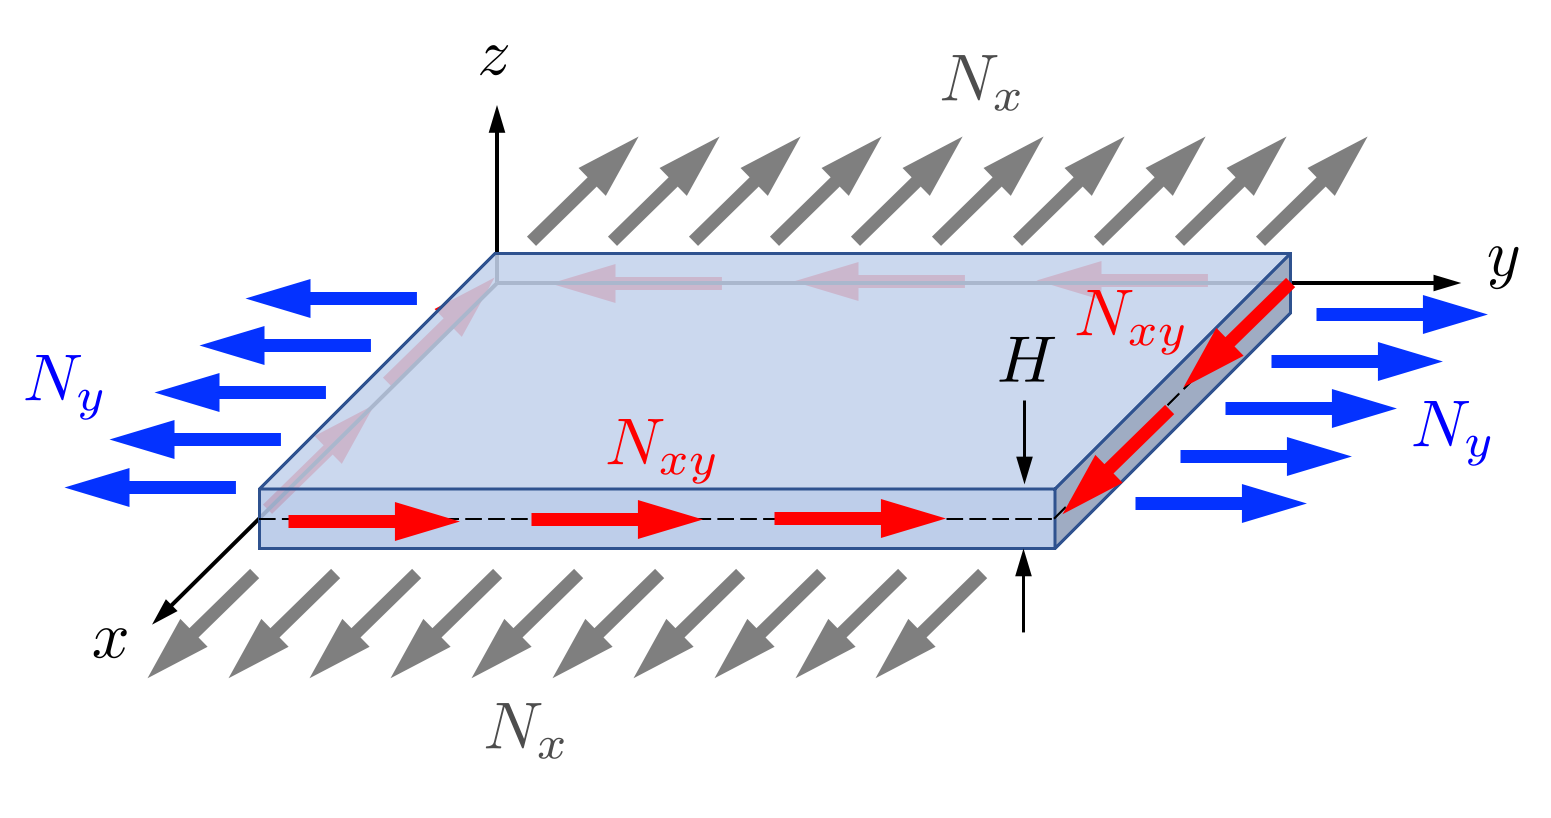
\includegraphics[width = 0.48\textwidth, trim = 10  00 10 10, clip = true, keepaspectratio = true]{Nlaminate.png}
   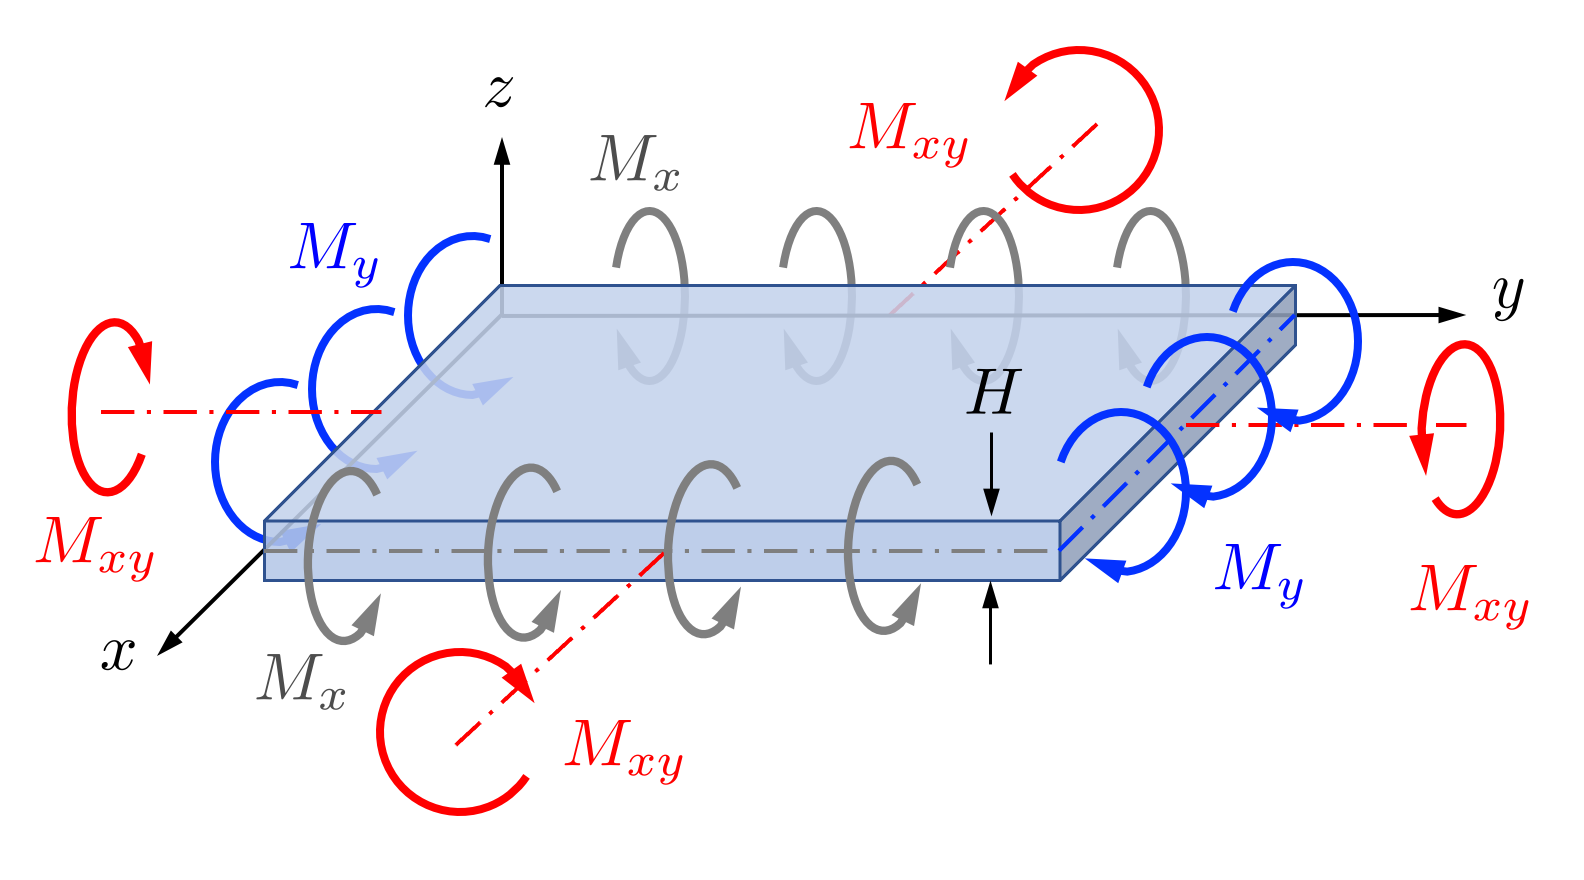
\includegraphics[width = 0.50\textwidth, trim = 10  15 10 10, clip = true, keepaspectratio = true]{Mlaminate.png}
   \caption{The in-plane loads per unit width (left) and moments per unit width (right) on a laminate.}
   \label{Nfig}
\end{figure}


Similarly, the vector of moments per unit width $\{M\}$ is defined as
\begin{equation}
   \left\{ \begin{array}{c}
     M_x \\ M_y \\ M_{xy}
   \end{array} \right\}
   = \bigintss_{-H/2}^{H/2} 
    \left\{ \begin{array}{c}
           \sigma_{xx}  \\  \sigma_{yy}  \\   \sigma_{xy}
           \end{array} \right\}
      z \ud z
  \label{Mdef}
\end{equation}
These are also sketched in Fig.~\ref{Nfig}, where you can see that $M_x$ and $M_y$ are bending moments, while $M_{xy}$ is a twisting moment in the $x$--$y$ coordinate system.  



\subsection*{Kirchoff-Love Hypothesis}

We would like to relate $\{ N \}$ and $\{ M \}$ to the deformation of the laminate.  To do this, classical lamination theory uses the Kirchoff-Love hypothesis.  This states that any material line initially normal to the $x$--$y$ plane remains straight and normal during deformation.  This is the laminated-plate analogy of slender beam theory.  However, while both a plate and a beam can bend in response to $M_x$, a plate can also bend in response to $M_y$ and twist in response to $M_{xy}$.  

With this hypothesis, the in-plane strains at any height $z$ are related to the strains on the midplane, which are $\varepsilon^0_{xx}$, $\varepsilon^0_{yy}$, and $\gamma^0_{xy}$, and to the midplane curvatures by
\begin{equation}
\renewcommand\arraystretch{1.2}
        \left\{ \begin{array}{c}
           \varepsilon_{xx}  \\  \varepsilon_{yy}  \\  \gamma_{xy}
           \end{array} \right\}
           =
        \left\{ \begin{array}{c}
           \varepsilon^0_{xx}  \\  \varepsilon^0_{yy}  \\  \gamma^0_{xy}
           \end{array} \right\}
           + z
        \left\{ \begin{array}{c}
           \kappa_{xx}  \\  \kappa_{yy}  \\  \kappa_{xy}
           \end{array} \right\}
     \label{Kirchoff}
\end{equation}
In the absence of curvature, every layer in a laminate has the same in-plane strain.  With curvature, strain increases linearly with $z$, in proportion to the corresponding component of curvature.  For example, a positive $\kappa_{xx}$ stretches the layers above the midplane, and compresses the layers below the midplane.  

\subsection*{Laminate Stiffness Equations}

Equations~(\ref{laminaQ}--\ref{Kirchoff}) can be combined to write an overall relationship between the forces and moments on the laminate and its midplane strains and curvatures.  That equation is
\begin{equation}
\renewcommand\arraystretch{1.2}
   \left\{ \begin{array}{c}
     N_x \\ N_y \\ N_{xy} \\  M_x \\ M_y \\ M_{xy}
   \end{array} \right\}
   =
\renewcommand\arraystretch{2}
   \left[ \begin{array}{c|c}
            A & B \\
            \hline
            B & D
      \end{array} \right]
\renewcommand\arraystretch{1.2}
        \left\{ \begin{array}{c}
           \varepsilon^0_{xx}  \\  \varepsilon^0_{yy}  \\  \gamma^0_{xy}  \\ \kappa_{xx}  \\  \kappa_{yy}  \\  \kappa_{xy}
           \end{array} \right\}
     \label{laminateStiffness}     
\end{equation}
The $6 \times 6$ matrix on the right-hand side of this equation contains several $3 \times 3$ sub-matrices, which are defined as
\begin{align}
     [A] &= \int_{-H/2}^{H/2} \: [Q(z)] \: \ud z  \label{Amatrix} \\
     [B] &= \int_{-H/2}^{H/2} \: [Q(z)] \: z \ud z \label{Bmatrix}  \\
     [D] &= \int_{-H/2}^{H/2}\: [Q(z)] \: z^2 \ud z  \label{Dmatrix}
\end{align}
The plane-strain stiffness matrix $[Q]$ is a function of $z$ because different layers have different fiber orientation.  We can see that $[A]$ relates the midplane strains to the in-plane loads $\{ N \}$, while $[D]$ relates the the midplane curvatures to the moments $\{ M \}$.  The $[B]$ matrix describes coupling, either between curvature and in-plane loads or between in-plane strains and moments.  If the laminate is symmetric about the midplane, i.e., if $[Q(z)] = [Q(-z)]$, then $[B] = 0$ and there is no coupling.  

To compute these matrices in a practical situation (and in \texttt{Clayer2laminate}), divide the laminate into $n$ discrete layers, and treat each layer as having a uniform $[Q]$.  Number the layers $i = 1$ to $n$ from the bottom of the laminate to the top, and let $[Q_i]$ be the plane-strain stiffness matrix for layer $i$.  Define $z_i$ such that layer $i$ extends from $z_{i-1}$ to $z_{i}$, with $z_0 = -H/2$ and $z_n = H/2$.  Now Eqns.~(\ref{Amatrix}--\ref{Dmatrix}) can be integrated analytically for each layer, and the matrices computed as
\begin{align}
     [A] &= \sum_{i=1}^n \: [Q_i] \: \left( z_i - z_{i-1} \right)  \label{Asum} \\
     [B] &= \sum_{i=1}^n  \: [Q_i] \: \left( \frac{z^2_i - z^2_{i-1}}{2} \right)  \label{Bsum}  \\
     [D] &= \sum_{i=1}^n  \: [Q_i] \: \left( \frac{z^3_i - z^3_{i-1}}{3} \right)  \label{Dsum}
\end{align}
$[A]$, $[B]$ and $[D]$ fully describe the elastic behavior of the laminate, and they are returned by \texttt{Clayer2laminate}.  

\subsection*{Extracting Tensile and Flexural Moduli}

As discussed in Section~8.1.5, any engineering constant like Young's modulus is defined in terms of a mechanical test where loads are applied and deformations are measured.  For the tensile modulus in the $x$ direction, a stress $\sigma_{xx}$ is applied, with all other stresses equal to zero, and the modulus is the ratio of the applied stress to $\varepsilon_{xx}$.  For a laminate we'll used the midplane strain, and also require that there be no moments applied.  Then, the $x$-direction tensile modulus is
\begin{equation}
    E^t_{xx} = \frac{\sigma_{xx}}{\varepsilon^0_{xx}}   = \frac{N_{x}/H}{\varepsilon^0_{xx}} 
    \label{EtensileDef}
 \end{equation}
We have used a superscript $t$ to indicate that this is a tensile modulus, and the second expression replaces the average stress $\sigma_{xx}$ with the load per unit width $N_x$.  A similar expression gives the $y$-direction tensile modulus.

To find the flexural modulus in the $x$ direction, one subjects the sample to a bending test where a moment $M_x$ is applied, with no other loads or moments, and the curvature $\kappa_{xx}$ is determined by measuring the deflection.  If this test were performed on a homogeneous beam of width $b$ and thickness $H$, the moment-curvature relationship would be
\begin{equation}
   M_x b = E^f_{xx} I \, \kappa_{xx} = \frac{E^f_{xx} b H^3}{12} \kappa_{xx}
   \label{momentCurvature}
\end{equation}
Here $I = bH^3/12$ is the moment of inertia of the cross-section, and the superscript $f$ on $E$ indicates a flexural modulus.  Note that $M_x$ is a moment per unit width, so the total applied moment is $M_x b$.  We can cancel $b$ from both sides and rearrange this equation to get the effective flexural modulus,
\begin{equation}
   E^f_{xx} = \frac{12 M_x}{H^3 \kappa_{xx}}
   \label{EflexDef}
\end{equation}
Analogous equations apply in the $y$ direction.  

To apply these results to a specific laminate, we need to find the midplane strain and the midplane curvature for the two load cases.  To do this numerically, invert the $6 \times 6$ matrix from the right-hand side of Eqn.~(\ref{laminateStiffness}).  The resulting matrix seems to have no official title, so we'll call it the laminate compliance matrix $[S^\mathrm{lam}]$:
\begin{equation}
    [S^\mathrm{lam}] 
    = 
   \left[ \begin{array}{c|c}
            A & B \\
            \hline
            B & D
      \end{array} \right] ^{-1}
   \label{SlamDef}
\end{equation}
Now the strain-stress relationship for the laminate is
\begin{equation}
\renewcommand\arraystretch{1.2}
        \left\{ \begin{array}{c}
           \varepsilon^0_{xx}  \\  \varepsilon^0_{yy}  \\  \gamma^0_{xy}  \\ \kappa_{xx}  \\  \kappa_{yy}  \\  \kappa_{xy}
           \end{array} \right\}
           = [S^\mathrm{lam}] 
\renewcommand\arraystretch{1.2}
   \left\{ \begin{array}{c}
     N_x \\ N_y \\ N_{xy} \\  M_x \\ M_y \\ M_{xy}
   \end{array} \right\}
     \label{laminateCompliance}     
\end{equation}
For a tensile test, with all loads and moments zero except $N_x$, the midplane strain is $\varepsilon^0_{xx} = S^\mathrm{lam}_{11} N_x$.  Using this in Eqn.~(\ref{EtensileDef}), we can calculate the laminate's tensile modulus in the $x$ direction as
\begin{equation}
     E^t_{xx} = \frac{1}{S^\mathrm{lam}_{11} H} 
     \label{EtxxFinal}
 \end{equation}
 Similarly, the tensile modulus in the $y$ direction is
\begin{equation}
     E^t_{yy} = \frac{1}{S^\mathrm{lam}_{22} H} 
     \label{EtyyFinal}
 \end{equation}
 For a bending test in the $x$ direction, the moment and curvature are related by $\kappa_{xx} = S^\mathrm{lam}_{44} M_x$.  Substituting this into Eqn.~(\ref{EflexDef}), we obtain an equation for the flexural modulus of the laminate in the $x$ direction,
 \begin{equation}
     E^f_{xx} = \frac{12}{S^\mathrm{lam}_{44} H^3}
     \label{EfxxFinal}
\end{equation}
The $y$-direction flexural modulus is found similarly,
 \begin{equation}
     E^f_{yy} = \frac{12}{S^\mathrm{lam}_{55} H^3}
     \label{EfyyFinal}
\end{equation}
 Equations~(\ref{EtxxFinal}--\ref{EfyyFinal}) are implemented in \texttt{Clayer2laminate}.  
  For an example calculation, see \break \texttt{LaminatedPlateProperties.mlx}.


\end{document}